%----------------------------------------------------------------------------------------
%	PACKAGES AND DOCUMENT CONFIGURATIONS
%----------------------------------------------------------------------------------------

\documentclass{article}


\usepackage{graphicx} % Required for the inclusion of images
\usepackage{subfigure} % Required for the inclusion of images
\usepackage{natbib} % Required to change bibliography style to APA
\usepackage{amsmath} % Required for some math elements 
\usepackage{listings}
\usepackage{float}
\usepackage[bookmarks=true,breaklinks,colorlinks,linkcolor=black,citecolor=black,urlcolor=black]{hyperref}


\lstset{frame=shadowbox,
	numbers=left,
	numberstyle=\scriptsize, basicstyle=\scriptsize	
}


%\usepackage{times} % Uncomment to use the Times New Roman font

%----------------------------------------------------------------------------------------
%	DOCUMENT INFORMATION
%----------------------------------------------------------------------------------------

\title{\textbf{Project 1: Optimizing the Performance of a Pipelined Processor}} % Title

\author{518030990028, TAKEHIRO MATSUNAGA, matsunagatakehiro@sjtu.edu.cn \\
        518030990025, EDUARDO WANG ZHENG, eduardo@sjtu.edu.cn \\
     } % Author name and email

\date{\today} % Date for the report

\begin{document}

\maketitle % Insert the title, author and date

\section{Introduction}

This project is divided into three parts: part A , B and C. \\

In part A, we write and simulate the following three Y86 programs: \textbf{sum.ys}, which iteratively sums linked list elements. \textbf{rsum.ys}, which recursively sums linked list elements. \textbf{copy.ys}, which copies a source block to a destination block. My partner writes and simulates \textbf{sum.ys} successfully first. After that, I and my partner writes and simulates \textbf{rsum.ys} and \textbf{copy.ys} separately, both succeed. \\

In part B, we modify the file \textbf{seq-full.hcl} to add new instruction. My partner also start first but get stuck when debugging at the GUI mode. I debug the same code and finally work it out.\\

In part C, I first modify \textbf{pipe-full.hcl} to add new instruction. After that, we modify \textbf{ncopy.ys} together. \\ \\
\textbf{Arrangement}:\\
TAKEHIRO MATSUNAGA: Part A, Part B,including corresponding experiment report,  \LaTeX \ layout and conclusion\\ \\
EDUARDO WANG ZHENG: Introduction and Part C,includining corresponding experiment report, conclusion.



\section{Experiments}

\subsection{Part A}

\subsubsection{Analysis}
%(a)\ \textbf{sum.ys}\\
First pass the pointer of array to function and initialize \textbf{\%eax}, which denotes \textbf{sum}. And judge wether the array is empty(the first value or address is zero). If it is, finish the function, or add the element to \textbf{sum}. Then get the next address which is four bytes after the element. If address is zero, finish or continue to loop. Finally when the loop is done, return the value by \textbf{\%eax}.\\ \\
(b)\ \textbf{rsum.ys}\\
First pass the pointer of array to function and initialize \textbf{\%eax}, which denotes \textbf{sum}. Line-30,Save the \textbf{\%ebp} which is the current element pointer(will be used in recurrence). And see whether the next address is legal. If it is zero, jump out of the function, and stop recurrence. If not save push the current pointer which point to the element now, then call \textbf{rsum\_list} itself again. As long as the recurrence stop, the pointers in stack will be popped and all element each pointer point to will be summed.\\ \\
(c)\ \textbf{copy.ys}\\
Push three argument in stack and call function. In function, get them from stack. Reading from source and writing to destination until the length becomes 0. Whenever succeed to read and write the length will decrease 1.
\subsubsection{Code}
%\rule{\textwidth}{0.3mm}
(a)\ \textbf{sum.ys}
\begin{lstlisting}
# code is written by TAKEHIRO MATSUNAGA
# Student ID: 518030990028
# sum.ys
# Execution begins at address 0 
.pos 0 
init:	irmovl Stack, %esp  	# Set up stack pointer  
irmovl Stack, %ebp  	# Set up base pointer   
call Main		# Execute main program
halt

#sample list array
.align 4
ele1:
.long 0x00a
.long ele2
ele2:	.long 0x0b0
.long ele3
ele3:	.long 0xc00
.long 0

# MAIN function
Main:	
irmovl ele1 , %esi	# array ptr -> source index
call sum_list
ret

# function--int sum_list(list_ptr ls)
# return value to %eax
sum_list:
irmovl $0, %eax		# %eax is sum
mrmovl (%esi), %ebx
andl %ebx, %ebx
je L2			# no element in array
L1:	mrmovl (%esi), %ebx
addl %ebx, %eax		# add to sum
mrmovl 4(%esi), %ebx
andl %ebx, %ebx
je L2			# whether array is finish
rrmovl %ebx, %esi	# next
jmp L1
L2:	ret

# The stack starts here and grows to lower addresses
.pos 0x100		
Stack:	  	 
\end{lstlisting}
(b)\ \textbf{rsum.ys}
\begin{lstlisting}
# code is written by TAKEHIRO MATSUNAGA
# Student ID: 518030990028
# rsum.ys
# Execution begins at address 0 
.pos 0 
init:	irmovl Stack, %esp 
irmovl Stack, %ebp 
call Main
halt

#sample list array
.align 4
ele1:
.long 0x00a
.long ele2
ele2:	.long 0x0b0
.long ele3
ele3:	.long 0xc00
.long 0

# MAIN function
Main:	irmovl ele1, %esi
irmovl $0, %eax
pushl %esi
call rsum_list
ret

# function--int rsum_list(list_ptr ls)
rsum_list:
pushl %ebp		# protect ret address and save bp
rrmovl %esp, %ebp	# stack handle
mrmovl 8(%ebp), %esi	# %esi get arg

andl %esi, %esi		# if zero or addr
je ZERO

rrmovl %esi, %ebp	# save %ebp
mrmovl 4(%esi), %esi	# next
pushl %esi
call rsum_list		# func call
popl %esi		# right sp
mrmovl (%ebp), %ebx	# %ebx = value
addl %ebx, %eax
jmp FIN			# loop

ZERO:	irmovl $0, %eax
FIN:	popl %ebp
ret

# The stack starts here and grows to lower addresses
.pos 0x200		
Stack:	 
\end{lstlisting}
(c)\ \textbf{copy.ys}
\begin{lstlisting}
# code is written by TAKEHIRO MATSUNAGA
# Student ID: 518030990028
# copy.ys
# Execution begins at address 0 
.pos 0 
init:	irmovl Stack, %esp 
irmovl Stack, %ebp 
call Main
halt

.align 4
# Source block
src:
.long 0x00a
.long 0x0b0
.long 0xc00
# Destination block
dest:
.long 0x111
.long 0x222
.long 0x333

# MAIN function
Main:	
irmovl src, %esi
irmovl dest, %edi
irmovl $3, %eax
pushl %esi
pushl %edi
pushl %eax
call copy_block
ret

# function--int copy_block(int *src, int *dest, int len)
copy_block:
pushl %ebp
rrmovl %esp, %ebp

mrmovl 8(%ebp), %ebx
mrmovl 12(%ebp), %edi
mrmovl 16(%ebp), %esi	# get arg from stack

irmovl $0, %eax		# %eax = result
andl %ebx, %ebx		# len == 0?
je ZERO
L1:	
mrmovl (%esi), %edx	# get elem from src
rmmovl %edx, (%edi)	# write elem to dst
irmovl $4, %ecx
addl %ecx, %edi
addl %ecx, %esi		# next elem of src, dst
xorl %edx, %eax		# xor chexk sum
irmovl $-1, %ecx	
addl %ecx, %ebx		# len --
jne L1

ZERO:	popl %ebp
ret

# The stack starts here and grows to lower addresses
.pos 0x100		
Stack:	 
\end{lstlisting}
\subsubsection{Evaluation}
\begin{figure}[H]
	\begin{minipage}[h]{\textwidth}
		\centering
		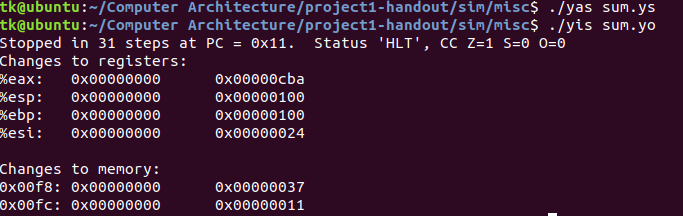
\includegraphics[width=0.9\textwidth]{sum_result.png}
		\caption{result of \textbf{sum.ys}} \label{Fig-G1}
		\hspace{5mm}
		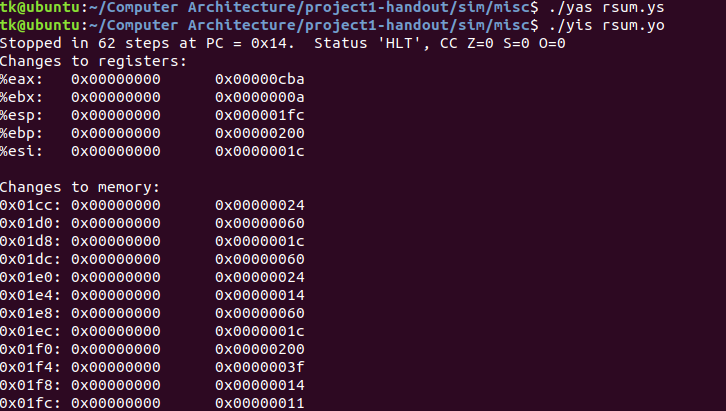
\includegraphics[width=0.9\textwidth]{rsum_result.png}
		\caption{result of \textbf{rsum.ys}} \label{Fig-G2}
		\hspace{5mm}
		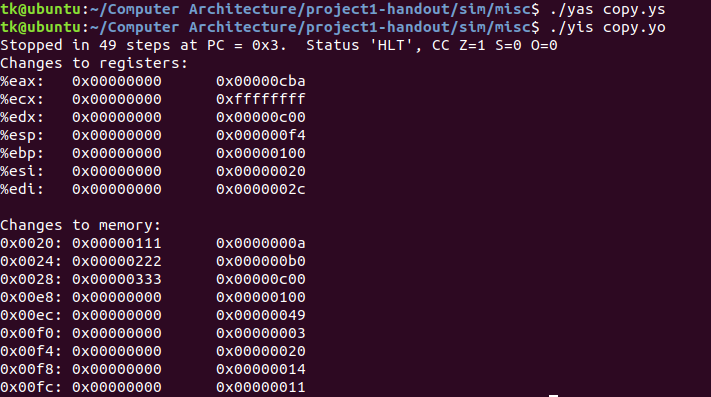
\includegraphics[width=0.9\textwidth]{copy_result.png}
		\caption{result of \textbf{copy.ys}} \label{Fig-G3}
	\end{minipage}
\end{figure}

\subsection{Part B}

\subsubsection{Analysis}
\begin{table}[H]
	\centering
	\begin{tabular}{p{5cm}p{5cm}}
		\hline
		stage	&iaddl V, rB\\
		\hline
		fetch:	&icode:ifun $\leftarrow $ M$_1$[PC]\\
				&rA:rB $\leftarrow$ M$_1$[PC+1]\\
				&valC $\leftarrow$ M$_4$[PC+2]\\
				&valP $\leftarrow$ PC + 6\\
		\\
		decode: &valB $\leftarrow$ R[rB]\\
		\\
		execute:&valE $\leftarrow$ valC + valB\\
				&Set CC\\
		\\
		memory: \\
		\\
		write back:&R[rB] $\leftarrow$ valE\\
		\\
		PC update:& PC $\leftarrow$ valP\\
		\hline
	\end{tabular}
\end{table}
\textbf{iaddl} is the operation which add an immediate and a number in register and put result in the register. So we know the instruction is 6 byte because it has immediate. \textbf{rA} is 0xfH in instruction code which is trivial. We just consider \textbf{rB} which pass to \textbf{ALU B} and immediate which pass to \textbf{ALU A}. Adding them and do not forget to change the flag condition state, which is \textbf{Set CC} in this stage. Write back to \textbf{rB} and go to next instruction.

\subsubsection{Code}

\begin{lstlisting}[numberstyle=\scriptsize, basicstyle=\scriptsize]
#code is rewritten by TAKEHIRO MATSUNAGA
#Student ID: 518030990028
#/* $begin seq-all-hcl */
####################################################################
#  HCL Description of Control for Single Cycle Y86 Processor SEQ   #
#  Copyright (C) Randal E. Bryant, David R. O'Hallaron, 2010       #
####################################################################

## Your task is to implement the iaddl instruction
## The file contains a declaration of the icodes
## for iaddl (IIADDL) .
## Your job is to add the rest of the logic to make it work

####################################################################
#    C Include's.  Don't alter these                               #
####################################################################

quote '#include <stdio.h>'
quote '#include "isa.h"'
quote '#include "sim.h"'
quote 'int sim_main(int argc, char *argv[]);'
quote 'int gen_pc(){return 0;}'
quote 'int main(int argc, char *argv[])'
quote '  {plusmode=0;return sim_main(argc,argv);}'

####################################################################
#    Declarations.  Do not change/remove/delete any of these       #
####################################################################

##### Symbolic representation of Y86 Instruction Codes #############
intsig INOP 	'I_NOP'
intsig IHALT	'I_HALT'
intsig IRRMOVL	'I_RRMOVL'
intsig IIRMOVL	'I_IRMOVL'
intsig IRMMOVL	'I_RMMOVL'
intsig IMRMOVL	'I_MRMOVL'
intsig IOPL	'I_ALU'
intsig IJXX	'I_JMP'
intsig ICALL	'I_CALL'
intsig IRET	'I_RET'
intsig IPUSHL	'I_PUSHL'
intsig IPOPL	'I_POPL'
# Instruction code for iaddl instruction
intsig IIADDL	'I_IADDL'

##### Symbolic represenations of Y86 function codes                  #####
intsig FNONE    'F_NONE'        # Default function code

##### Symbolic representation of Y86 Registers referenced explicitly #####
intsig RESP     'REG_ESP'    	# Stack Pointer
intsig REBP     'REG_EBP'    	# Frame Pointer
intsig RNONE    'REG_NONE'   	# Special value indicating "no register"

##### ALU Functions referenced explicitly                            #####
intsig ALUADD	'A_ADD'		# ALU should add its arguments

##### Possible instruction status values                             #####
intsig SAOK	'STAT_AOK'		# Normal execution
intsig SADR	'STAT_ADR'	# Invalid memory address
intsig SINS	'STAT_INS'	# Invalid instruction
intsig SHLT	'STAT_HLT'	# Halt instruction encountered

##### Signals that can be referenced by control logic ####################

##### Fetch stage inputs		#####
intsig pc 'pc'				# Program counter
##### Fetch stage computations		#####
intsig imem_icode 'imem_icode'		# icode field from instruction memory
intsig imem_ifun  'imem_ifun' 		# ifun field from instruction memory
intsig icode	  'icode'		# Instruction control code
intsig ifun	  'ifun'		# Instruction function
intsig rA	  'ra'			# rA field from instruction
intsig rB	  'rb'			# rB field from instruction
intsig valC	  'valc'		# Constant from instruction
intsig valP	  'valp'		# Address of following instruction
boolsig imem_error 'imem_error'		# Error signal from instruction memory
boolsig instr_valid 'instr_valid'	# Is fetched instruction valid?

##### Decode stage computations		#####
intsig valA	'vala'			# Value from register A port
intsig valB	'valb'			# Value from register B port

##### Execute stage computations	#####
intsig valE	'vale'			# Value computed by ALU
boolsig Cnd	'cond'			# Branch test

##### Memory stage computations		#####
intsig valM	'valm'			# Value read from memory
boolsig dmem_error 'dmem_error'		# Error signal from data memory

####################################################################
#    Control Signal Definitions.                                   #
####################################################################

################ Fetch Stage     ###################################

# Determine instruction code
int icode = [
imem_error: INOP;
1: imem_icode;		# Default: get from instruction memory
];

# Determine instruction function
int ifun = [
imem_error: FNONE;
1: imem_ifun;		# Default: get from instruction memory
];

bool instr_valid = icode in 
{ INOP, IHALT, IRRMOVL, IIRMOVL, IRMMOVL, IMRMOVL,
IOPL, IJXX, ICALL, IRET, IPUSHL, IPOPL, IIADDL };

# Does fetched instruction require a regid byte?
bool need_regids =
icode in { IRRMOVL, IOPL, IPUSHL, IPOPL, 
IIRMOVL, IRMMOVL, IMRMOVL, IIADDL };

# Does fetched instruction require a constant word?
bool need_valC =
icode in { IIRMOVL, IRMMOVL, IMRMOVL, IJXX, ICALL, IIADDL };

################ Decode Stage    ###################################

## What register should be used as the A source?
int srcA = [
icode in { IRRMOVL, IRMMOVL, IOPL, IPUSHL  } : rA;
icode in { IPOPL, IRET } : RESP;
1 : RNONE; # Don't need register
];

## What register should be used as the B source?
int srcB = [
icode in { IOPL, IRMMOVL, IMRMOVL, IIADDL  } : rB;
icode in { IPUSHL, IPOPL, ICALL, IRET } : RESP;
1 : RNONE;  # Don't need register
];

## What register should be used as the E destination?
int dstE = [
icode in { IRRMOVL } && Cnd : rB;
icode in { IIRMOVL, IOPL, IIADDL} : rB;
icode in { IPUSHL, IPOPL, ICALL, IRET } : RESP;
1 : RNONE;  # Don't write any register
];

## What register should be used as the M destination?
int dstM = [
icode in { IMRMOVL, IPOPL } : rA;
1 : RNONE;  # Don't write any register
];

################ Execute Stage   ###################################

## Select input A to ALU
int aluA = [
icode in { IRRMOVL, IOPL } : valA;
icode in { IIRMOVL, IRMMOVL, IMRMOVL, IIADDL } : valC;
icode in { ICALL, IPUSHL } : -4;
icode in { IRET, IPOPL } : 4;
# Other instructions don't need ALU
];

## Select input B to ALU
int aluB = [
icode in { IRMMOVL, IMRMOVL, IOPL, ICALL, 
IPUSHL, IRET, IPOPL, IIADDL } : valB;
icode in { IRRMOVL, IIRMOVL } : 0;
# Other instructions don't need ALU
];

## Set the ALU function
int alufun = [
icode == IOPL : ifun;
1 : ALUADD;
];

## Should the condition codes be updated?
bool set_cc = icode in { IOPL, IIADDL };

################ Memory Stage    ###################################

## Set read control signal
bool mem_read = icode in { IMRMOVL, IPOPL, IRET };

## Set write control signal
bool mem_write = icode in { IRMMOVL, IPUSHL, ICALL };

## Select memory address
int mem_addr = [
icode in { IRMMOVL, IPUSHL, ICALL, IMRMOVL } : valE;
icode in { IPOPL, IRET } : valA;
# Other instructions don't need address
];

## Select memory input data
int mem_data = [
# Value from register
icode in { IRMMOVL, IPUSHL } : valA;
# Return PC
icode == ICALL : valP;
# Default: Don't write anything
];

## Determine instruction status
int Stat = [
imem_error || dmem_error : SADR;
!instr_valid: SINS;
icode == IHALT : SHLT;
1 : SAOK;
];

################ Program Counter Update ############################

## What address should instruction be fetched at

int new_pc = [
# Call.  Use instruction constant
icode == ICALL : valC;
# Taken branch.  Use instruction constant
icode == IJXX && Cnd : valC;
# Completion of RET instruction.  Use value from stack
icode == IRET : valM;
# Default: Use incremented PC
1 : valP;
];
#/* $end seq-all-hcl */
\end{lstlisting}

\subsubsection{Evaluation}

\begin{figure}[H]
	\begin{minipage}[h]{\textwidth}
		\centering
		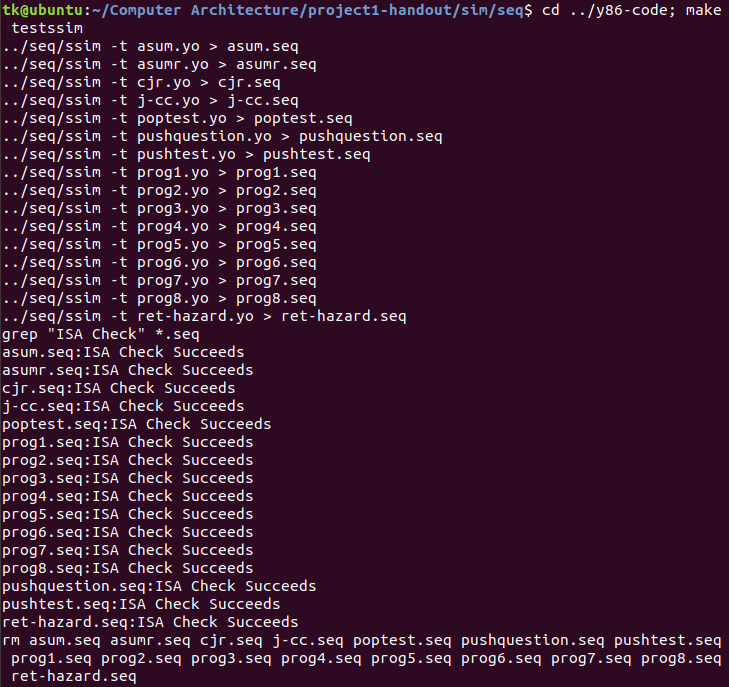
\includegraphics[width=1\textwidth]{seq_correctness.png}
		\caption{correctness test of \textbf{seq-full.hcl}} \label{Fig-G4}
		\hspace{5mm}
		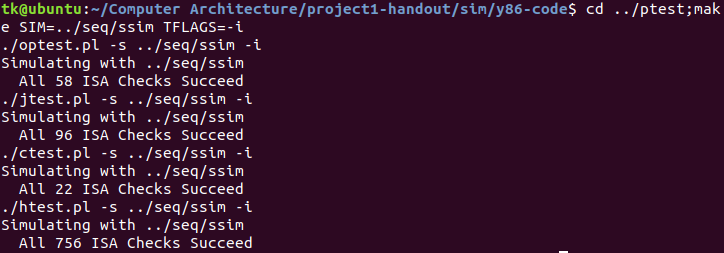
\includegraphics[width=1\textwidth]{seq_iaddl.png}
		\caption{\textbf{iaddl} test of \textbf{seq-full.hcl}} \label{Fig-G5}
	\end{minipage}
\end{figure}

\subsection{Part C}

\subsubsection{Analysis}

The task is consist of two parts: modify \textbf{pipe-full.hcl} to add new instruction., modify \textbf{ncopy.ys} to make it run faster. The first part is almost the same to modify the file seq-full.hcl, which is relevantly easy. So the key part is to modify \textbf{ncopy.ys}. After discussion, we mainly find two Optimization points:\\
1. Add the \textbf{iaddl} instruction, which is already done by modifying \textbf{pipe-full.hcl}. After that, we can replace the arithmetic operation with \textbf{iaddl}. At the same time, because \textbf{iaddl} has the step of \textbf{set CC}, the corresponding \textbf{andl} instruction is unnecessary.\\
2. Loop unrolling. Unroll by a factor of 4, we can Eliminate unnecessary instructions. Howerver, to handle the case that the number of elements is not divisible by 4, we need an extra loop(Loop2) that simply copy src to dst one by one and check if the element we have moved is valid in each test (test 1~5). If the element is valid, we increment the count\textbf{(\%eax)}.


\subsubsection{Code}
\textbf{pipe-full.hcl}
\begin{lstlisting}[numberstyle=\scriptsize, basicstyle=\scriptsize]
# Name: Eduardo Wang Zheng
# Student ID: 518030990025
#iaddl:
#   fetch:      f_icode:f_ifun <-- M1[PC]
#               D_rA:D_rB <-- M1[PC + 1]
#               E_valC <-- M4[PC + 2]
#               D_valP <-- PC + 6
#   decode:     E_valB <-- R[rB]
#   execute:    e_valE <-- E_valC + E_valB
#               Set CC
#   memory: 
#   write back: R[rB] <- e_valE
#   PC update:  PC <-- D_valP




#/* $begin pipe-all-hcl */
####################################################################
#    HCL Description of Control for Pipelined Y86 Processor        #
#    Copyright (C) Randal E. Bryant, David R. O'Hallaron, 2010     #
####################################################################

## Your task is to implement the iaddl and leave instructions
## The file contains a declaration of the icodes
## for iaddl (IIADDL) and leave (ILEAVE).
## Your job is to add the rest of the logic to make it work

####################################################################
#    C Include's.  Don't alter these                               #
####################################################################

quote '#include <stdio.h>'
quote '#include "isa.h"'
quote '#include "pipeline.h"'
quote '#include "stages.h"'
quote '#include "sim.h"'
quote 'int sim_main(int argc, char *argv[]);'
quote 'int main(int argc, char *argv[]){return sim_main(argc,argv);}'

####################################################################
#    Declarations.  Do not change/remove/delete any of these       #
####################################################################

##### Symbolic representation of Y86 Instruction Codes #############
intsig INOP 	'I_NOP'
intsig IHALT	'I_HALT'
intsig IRRMOVL	'I_RRMOVL'
intsig IIRMOVL	'I_IRMOVL'
intsig IRMMOVL	'I_RMMOVL'
intsig IMRMOVL	'I_MRMOVL'
intsig IOPL	'I_ALU'
intsig IJXX	'I_JMP'
intsig ICALL	'I_CALL'
intsig IRET	'I_RET'
intsig IPUSHL	'I_PUSHL'
intsig IPOPL	'I_POPL'
# Instruction code for iaddl instruction
intsig IIADDL	'I_IADDL'
# Instruction code for leave instruction
intsig ILEAVE	'I_LEAVE'

##### Symbolic represenations of Y86 function codes            #####
intsig FNONE    'F_NONE'        # Default function code

##### Symbolic representation of Y86 Registers referenced      #####
intsig RESP     'REG_ESP'    	     # Stack Pointer
intsig REBP     'REG_EBP'    	     # Frame Pointer
intsig RNONE    'REG_NONE'   	     # Special value indicating "no register"

##### ALU Functions referenced explicitly ##########################
intsig ALUADD	'A_ADD'		     # ALU should add its arguments

##### Possible instruction status values                       #####
intsig SBUB	'STAT_BUB'	# Bubble in stage
intsig SAOK	'STAT_AOK'	# Normal execution
intsig SADR	'STAT_ADR'	# Invalid memory address
intsig SINS	'STAT_INS'	# Invalid instruction
intsig SHLT	'STAT_HLT'	# Halt instruction encountered

##### Signals that can be referenced by control logic ##############

##### Pipeline Register F ##########################################

intsig F_predPC 'pc_curr->pc'	     # Predicted value of PC

##### Intermediate Values in Fetch Stage ###########################

intsig imem_icode  'imem_icode'      # icode field from instruction memory
intsig imem_ifun   'imem_ifun'       # ifun  field from instruction memory
intsig f_icode	'if_id_next->icode'  # (Possibly modified) instruction code
intsig f_ifun	'if_id_next->ifun'   # Fetched instruction function
intsig f_valC	'if_id_next->valc'   # Constant data of fetched instruction
intsig f_valP	'if_id_next->valp'   # Address of following instruction
boolsig imem_error 'imem_error'	     # Error signal from instruction memory
boolsig instr_valid 'instr_valid'    # Is fetched instruction valid?

##### Pipeline Register D ##########################################
intsig D_icode 'if_id_curr->icode'   # Instruction code
intsig D_rA 'if_id_curr->ra'	     # rA field from instruction
intsig D_rB 'if_id_curr->rb'	     # rB field from instruction
intsig D_valP 'if_id_curr->valp'     # Incremented PC

##### Intermediate Values in Decode Stage  #########################

intsig d_srcA	 'id_ex_next->srca'  # srcA from decoded instruction
intsig d_srcB	 'id_ex_next->srcb'  # srcB from decoded instruction
intsig d_rvalA 'd_regvala'	     # valA read from register file
intsig d_rvalB 'd_regvalb'	     # valB read from register file

##### Pipeline Register E ##########################################
intsig E_icode 'id_ex_curr->icode'   # Instruction code
intsig E_ifun  'id_ex_curr->ifun'    # Instruction function
intsig E_valC  'id_ex_curr->valc'    # Constant data
intsig E_srcA  'id_ex_curr->srca'    # Source A register ID
intsig E_valA  'id_ex_curr->vala'    # Source A value
intsig E_srcB  'id_ex_curr->srcb'    # Source B register ID
intsig E_valB  'id_ex_curr->valb'    # Source B value
intsig E_dstE 'id_ex_curr->deste'    # Destination E register ID
intsig E_dstM 'id_ex_curr->destm'    # Destination M register ID

##### Intermediate Values in Execute Stage #########################
intsig e_valE 'ex_mem_next->vale'	# valE generated by ALU
boolsig e_Cnd 'ex_mem_next->takebranch' # Does condition hold?
intsig e_dstE 'ex_mem_next->deste'      # dstE (possibly modified to be RNONE)

##### Pipeline Register M                  #########################
intsig M_stat 'ex_mem_curr->status'     # Instruction status
intsig M_icode 'ex_mem_curr->icode'	# Instruction code
intsig M_ifun  'ex_mem_curr->ifun'	# Instruction function
intsig M_valA  'ex_mem_curr->vala'      # Source A value
intsig M_dstE 'ex_mem_curr->deste'	# Destination E register ID
intsig M_valE  'ex_mem_curr->vale'      # ALU E value
intsig M_dstM 'ex_mem_curr->destm'	# Destination M register ID
boolsig M_Cnd 'ex_mem_curr->takebranch'	# Condition flag
boolsig dmem_error 'dmem_error'	        # Error signal from instruction memory

##### Intermediate Values in Memory Stage ##########################
intsig m_valM 'mem_wb_next->valm'	# valM generated by memory
intsig m_stat 'mem_wb_next->status'	# stat (possibly modified to be SADR)

##### Pipeline Register W ##########################################
intsig W_stat 'mem_wb_curr->status'     # Instruction status
intsig W_icode 'mem_wb_curr->icode'	# Instruction code
intsig W_dstE 'mem_wb_curr->deste'	# Destination E register ID
intsig W_valE  'mem_wb_curr->vale'      # ALU E value
intsig W_dstM 'mem_wb_curr->destm'	# Destination M register ID
intsig W_valM  'mem_wb_curr->valm'	# Memory M value

####################################################################
#    Control Signal Definitions.                                   #
####################################################################

################ Fetch Stage     ###################################

## What address should instruction be fetched at
int f_pc = [
# Mispredicted branch.  Fetch at incremented PC
M_icode == IJXX && !M_Cnd : M_valA;
# Completion of RET instruction.
W_icode == IRET : W_valM;
# Default: Use predicted value of PC
1 : F_predPC;
];

## Determine icode of fetched instruction
int f_icode = [
imem_error : INOP;
1: imem_icode;
];

# Determine ifun
int f_ifun = [
imem_error : FNONE;
1: imem_ifun;
];

# Is instruction valid?
bool instr_valid = f_icode in 
{ INOP, IHALT, IRRMOVL, IIRMOVL, IRMMOVL, IMRMOVL,
IOPL, IJXX, ICALL, IRET, IPUSHL, IPOPL, IIADDL}; #make IADDL valid



# Determine status code for fetched instruction
int f_stat = [
imem_error: SADR;
!instr_valid : SINS;
f_icode == IHALT : SHLT;
1 : SAOK;
];

# Does fetched instruction require a regid byte?
bool need_regids =
f_icode in  { IRRMOVL, IOPL, IPUSHL, IPOPL, 
IIRMOVL, IRMMOVL, IMRMOVL, IIADDL}; # IADDL requires a regid byte

# Does fetched instruction require a constant word?
bool need_valC =
f_icode in { IIRMOVL, IRMMOVL, IMRMOVL, IJXX, ICALL, IIADDL }; # IADDL requires a constant word


# Predict next value of PC
int f_predPC = [
f_icode in { IJXX, ICALL } : f_valC;
1 : f_valP;
];

################ Decode Stage ######################################


## What register should be used as the A source?
int d_srcA = [
D_icode in { IRRMOVL, IRMMOVL, IOPL, IPUSHL  } : D_rA;
D_icode in { IPOPL, IRET } : RESP;
1 : RNONE; # Don't need register
];

## What register should be used as the B source?
int d_srcB = [
D_icode in { IOPL, IRMMOVL, IMRMOVL, IIADDL  } : D_rB; #IADDL register should be used as the B source
D_icode in { IPUSHL, IPOPL, ICALL, IRET } : RESP;
1 : RNONE;  # Don't need register
];

## What register should be used as the E destination?
int d_dstE = [

D_icode in { IRRMOVL }&&e_Cnd  : D_rB;   #condition changes
D_icode in { IIRMOVL, IOPL, IIADDL} : D_rB; #IADDL register should be used as the E destination
D_icode in { IPUSHL, IPOPL, ICALL, IRET } : RESP;
1 : RNONE;  # Don't write any register
];

## What register should be used as the M destination?
int d_dstM = [
D_icode in { IMRMOVL, IPOPL } : D_rA;
1 : RNONE;  # Don't write any register
];

## What should be the A value?
## Forward into decode stage for valA
int d_valA = [
D_icode in { ICALL, IJXX } : D_valP; # Use incremented PC
d_srcA == e_dstE : e_valE;    # Forward valE from execute
d_srcA == M_dstM : m_valM;    # Forward valM from memory
d_srcA == M_dstE : M_valE;    # Forward valE from memory
d_srcA == W_dstM : W_valM;    # Forward valM from write back
d_srcA == W_dstE : W_valE;    # Forward valE from write back
1 : d_rvalA;  # Use value read from register file
];

int d_valB = [
d_srcB == e_dstE : e_valE;    # Forward valE from execute
d_srcB == M_dstM : m_valM;    # Forward valM from memory
d_srcB == M_dstE : M_valE;    # Forward valE from memory
d_srcB == W_dstM : W_valM;    # Forward valM from write back
d_srcB == W_dstE : W_valE;    # Forward valE from write back
1 : d_rvalB;  # Use value read from register file
];

################ Execute Stage #####################################

## Select input A to ALU
int aluA = [
E_icode in { IRRMOVL, IOPL } : E_valA;
E_icode in { IIRMOVL, IRMMOVL, IMRMOVL, IIADDL } : E_valC; #IADDL register uses input A to ALU
E_icode in { ICALL, IPUSHL } : -4;
E_icode in { IRET, IPOPL } : 4;
# Other instructions don't need ALU


# Other instructions don't need ALU
];

## Select input B to ALU
int aluB = [
E_icode in { IRMMOVL, IMRMOVL, IOPL, ICALL, 
IPUSHL, IRET, IPOPL, IIADDL } : E_valB; #IADDL register uses input B to ALU
E_icode in { IRRMOVL, IIRMOVL } : 0;
# Other instructions don't need ALU


];

## Set the ALU function
int alufun = [
E_icode == IOPL : E_ifun;
1 : ALUADD;
];

## Should the condition codes be updated?
bool set_cc = E_icode in { IOPL, IIADDL } &&
# State changes only during normal operation
!m_stat in { SADR, SINS, SHLT } && !W_stat in { SADR, SINS, SHLT }; #condition changes

## Generate valA in execute stage
int e_valA = E_valA;    # Pass valA through stage

## Set dstE to RNONE in event of not-taken conditional move
int e_dstE = [
E_icode == IRRMOVL && !e_Cnd : RNONE;
1 : E_dstE;
];

################ Memory Stage ######################################

## Select memory address
int mem_addr = [
M_icode in { IRMMOVL, IPUSHL, ICALL, IMRMOVL } : M_valE;
M_icode in { IPOPL, IRET } : M_valA;
# Other instructions don't need address
];

## Set read control signal
bool mem_read = M_icode in { IMRMOVL, IPOPL, IRET };

## Set write control signal
bool mem_write = M_icode in { IRMMOVL, IPUSHL, ICALL };

#/* $begin pipe-m_stat-hcl */
## Update the status
int m_stat = [
dmem_error : SADR;
1 : M_stat;
];
#/* $end pipe-m_stat-hcl */

## Set E port register ID
int w_dstE = W_dstE;

## Set E port value
int w_valE = W_valE;

## Set M port register ID
int w_dstM = W_dstM;

## Set M port value
int w_valM = W_valM;

## Update processor status
int Stat = [
W_stat == SBUB : SAOK;
1 : W_stat;
];

################ Pipeline Register Control #########################

# Should I stall or inject a bubble into Pipeline Register F?
# At most one of these can be true.
bool F_bubble = 0;
bool F_stall =
# Conditions for a load/use hazard
E_icode in { IMRMOVL, IPOPL } &&
E_dstM in { d_srcA, d_srcB } ||
# Stalling at fetch while ret passes through pipeline
IRET in { D_icode, E_icode, M_icode };

# Should I stall or inject a bubble into Pipeline Register D?
# At most one of these can be true.
bool D_stall = 
# Conditions for a load/use hazard
E_icode in { IMRMOVL, IPOPL } &&
E_dstM in { d_srcA, d_srcB };

bool D_bubble =
# Mispredicted branch
(E_icode == IJXX && !e_Cnd) ||
# Stalling at fetch while ret passes through pipeline
# but not condition for a load/use hazard
!(E_icode in { IMRMOVL, IPOPL } && E_dstM in { d_srcA, d_srcB }) &&
IRET in { D_icode, E_icode, M_icode };

# Should I stall or inject a bubble into Pipeline Register E?
# At most one of these can be true.
bool E_stall = 0;
bool E_bubble =
# Mispredicted branch
(E_icode == IJXX && !e_Cnd) ||
# Conditions for a load/use hazard
E_icode in { IMRMOVL, IPOPL } &&
E_dstM in { d_srcA, d_srcB};

# Should I stall or inject a bubble into Pipeline Register M?
# At most one of these can be true.
bool M_stall = 0;
# Start injecting bubbles as soon as exception passes through memory stage
bool M_bubble = m_stat in { SADR, SINS, SHLT } || W_stat in { SADR, SINS, SHLT };

# Should I stall or inject a bubble into Pipeline Register W?
bool W_stall = W_stat in { SADR, SINS, SHLT };
bool W_bubble = 0;
#/* $end pipe-all-hcl */
\end{lstlisting}
\quad \\
\textbf{ncopy.ys}
\begin{lstlisting}[numberstyle=\scriptsize, basicstyle=\scriptsize]
# Name: Eduardo Wang Zheng
# Student ID: 518030990025
#/* $begin ncopy-ys */
##################################################################
# ncopy.ys - Copy a src block of len ints to dst.
# Return the number of positive ints (>0) contained in src.
#
# Include your name and ID here.
#
# Describe how and why you modified the baseline code.
#
##################################################################
# Do not modify this portion
# Function prologue.
ncopy:	pushl %ebp		# Save old frame pointer
rrmovl %esp,%ebp	# Set up new frame pointer
pushl %esi		# Save callee-save regs
pushl %ebx
pushl %edi
mrmovl 8(%ebp),%ebx	# src
mrmovl 16(%ebp),%edx	# len
mrmovl 12(%ebp),%ecx	# dst

##################################################################
# You can modify this portion
# Loop header
xorl %eax,%eax      # count = 0;
iaddl $-3, %edx     # len- = 3
jle next_start      # if so, goto Done:

Loop1:  
mrmovl (%ebx), %esi # read val from src...
mrmovl 4(%ebx), %edi # read val from src + 1
rmmovl %esi, (%ecx) # ...and store it to dst
rmmovl %edi, 4(%ecx) # store it to dst + 1
test1:
andl %esi, %esi     # *src <= 0 ?
jle test2
iaddl $1, %eax      # count++
test2:
andl %edi, %edi     # *(src + 1) <= 0 ?
jle test3
iaddl $1, %eax      # count++
test3:
mrmovl 8(%ebx), %esi # read val from src + 2
mrmovl 12(%ebx), %edi # read val from src + 3
rmmovl %esi, 8(%ecx) # store it to dst + 2
rmmovl %edi, 12(%ecx) # store it to dst + 3
andl %esi, %esi     # *(src + 2) <= 0?
jle test4
iaddl $1, %eax      # count++
test4:
andl %edi, %edi     # *(src + 3) <= 0?
jle Npos
iaddl $1, %eax      # count++
Npos:
iaddl $16, %ebx     # src += 4
iaddl $16, %ecx     # dst += 4
iaddl $-4, %edx     # len -= 4
andl %edx,%edx      # len > 0?
jg Loop1            # if so, goto Loop:
next_start:
iaddl $3, %edx      # len += 3
jle Done
loop2:
mrmovl (%ebx), %esi # read val from src
rmmovl %esi, (%ecx) # store it to dst
andl %esi, %esi     # *src <= 0 ?
jle test5
iaddl $1, %eax      # count++
test5:
iaddl $4, %ebx      # src += 1
iaddl $4, %ecx      # dst += 1
iaddl $-1, %edx     # len -= 1
jg loop2
##################################################################
# Do not modify the following section of code
# Function epilogue.
Done:
popl %edi               # Restore callee-save registers
popl %ebx
popl %esi
rrmovl %ebp, %esp
popl %ebp
ret
##################################################################
# Keep the following label at the end of your function
End:
#/* $end ncopy-ys */
\end{lstlisting}

\subsubsection{Evaluation}

\begin{figure}[H]
	\begin{minipage}[h]{\textwidth}
		\centering
		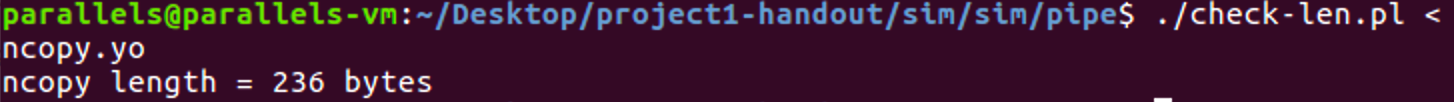
\includegraphics[width=1\textwidth]{length_check.png}
		\caption{length check.hcl} \label{Fig-G6}
		\hspace{5mm}
		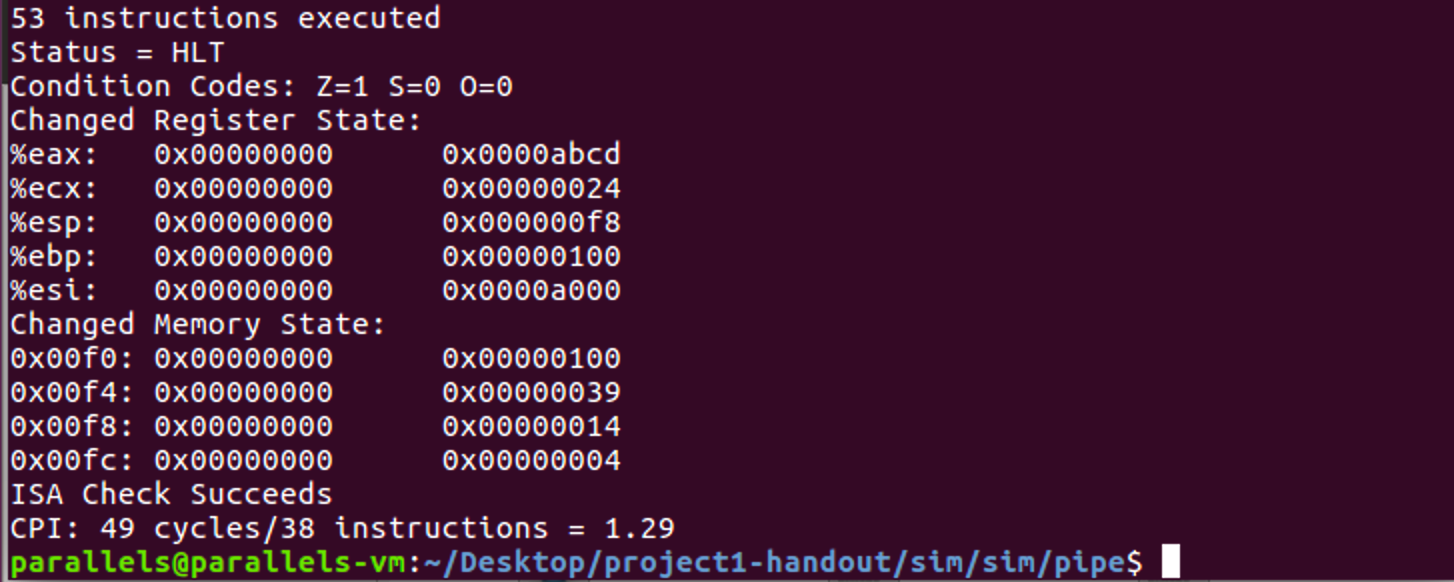
\includegraphics[width=1\textwidth]{execute_asumi.yo.png}
		\caption{Execute \textbf{asumi.yo}} \label{Fig-G7}
		\hspace{5mm}
		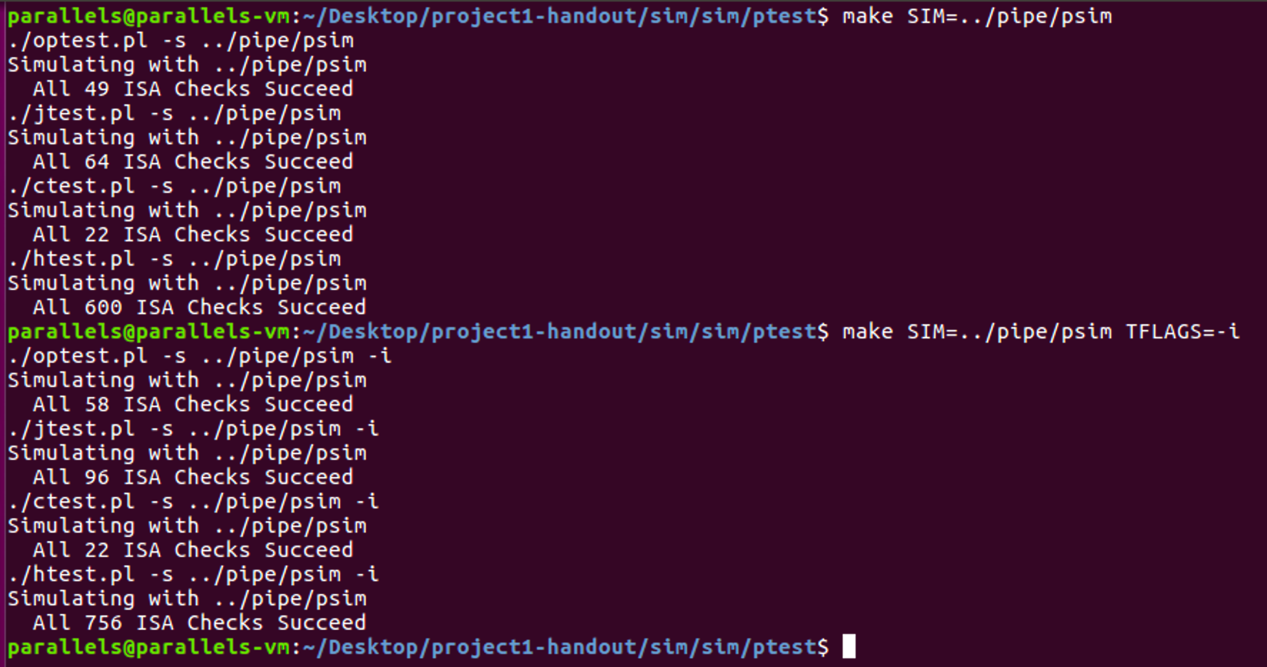
\includegraphics[width=1\textwidth]{regression_tests.png}
		\caption{Performing regression tests.} \label{Fig-G8}
		\hspace{5mm}
	\end{minipage}
\end{figure}
\begin{figure}[H]	
	\begin{minipage}[h]{\textwidth}	
		\centering
		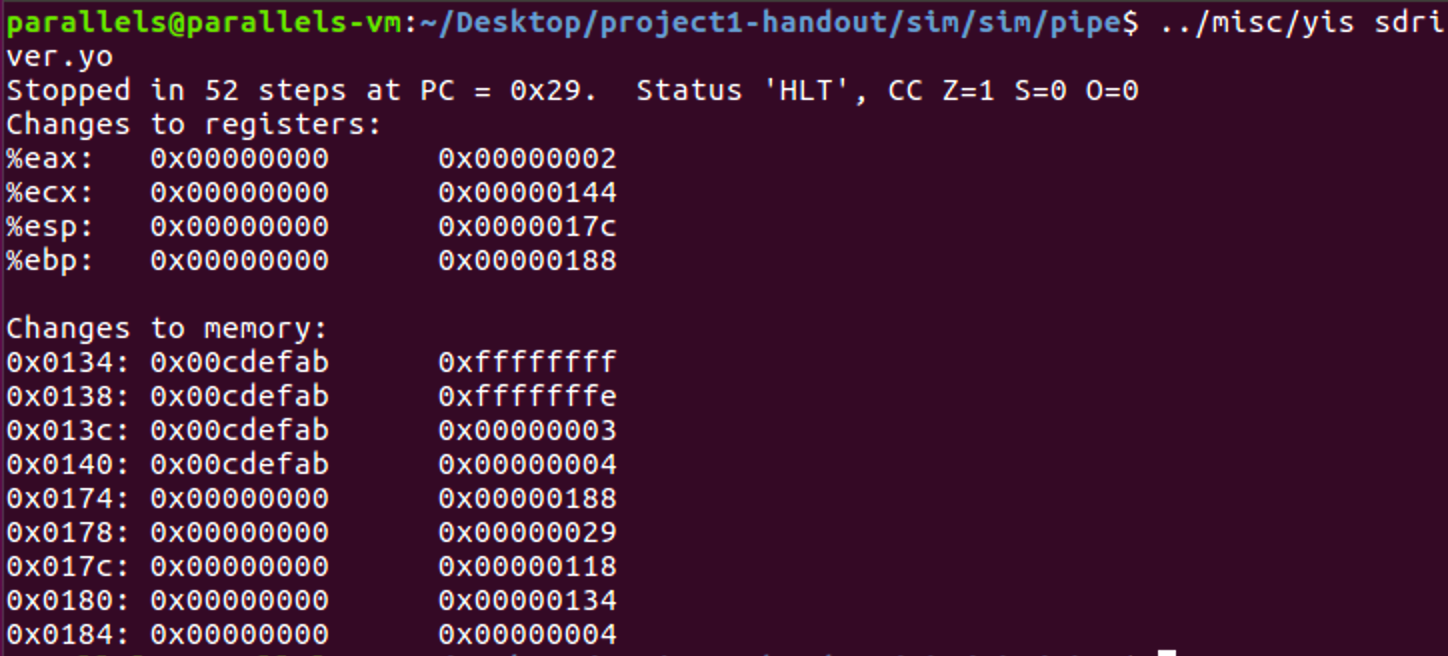
\includegraphics[width=1\textwidth]{driver_file_test.png}
		\caption{Testing driver files on the ISA simulator} \label{Fig-G9}
		\hspace{5mm}
		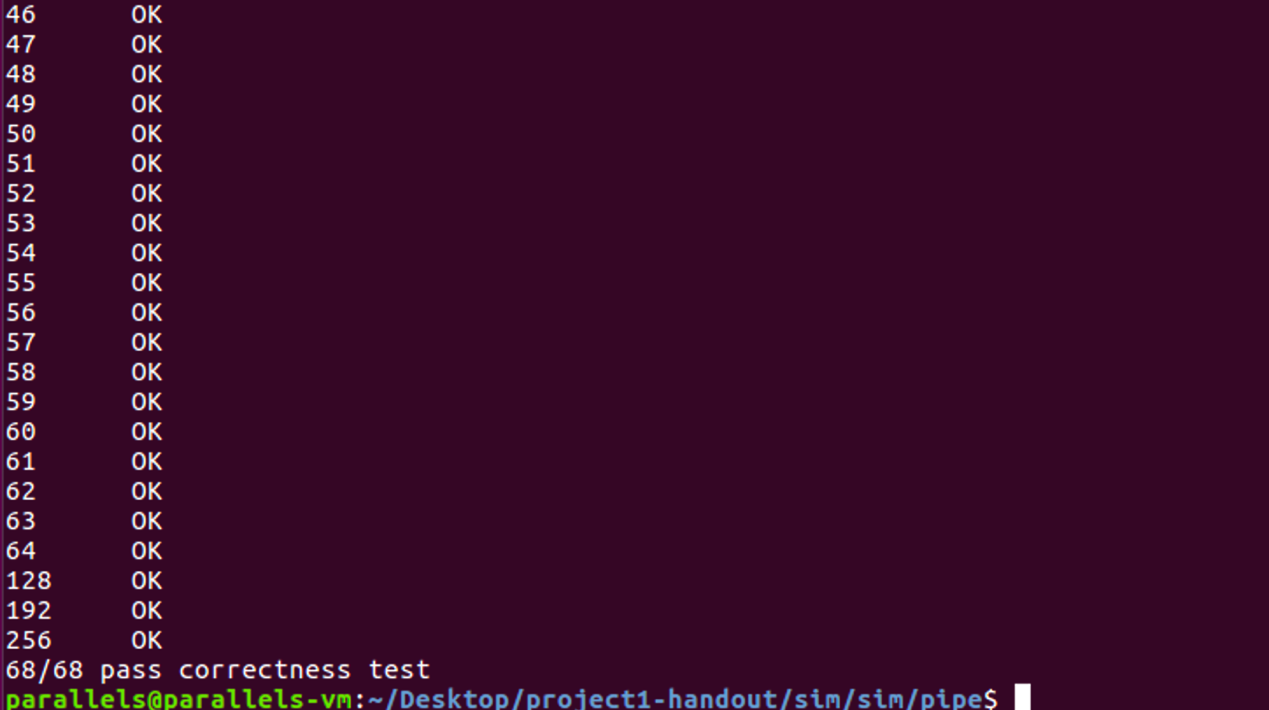
\includegraphics[width=1\textwidth]{arrang_block_test_ISA.png}
		\caption{Testing code on arrange of block lengths with the ISA simulator} \label{Fig-G10}
		\hspace{5mm}
		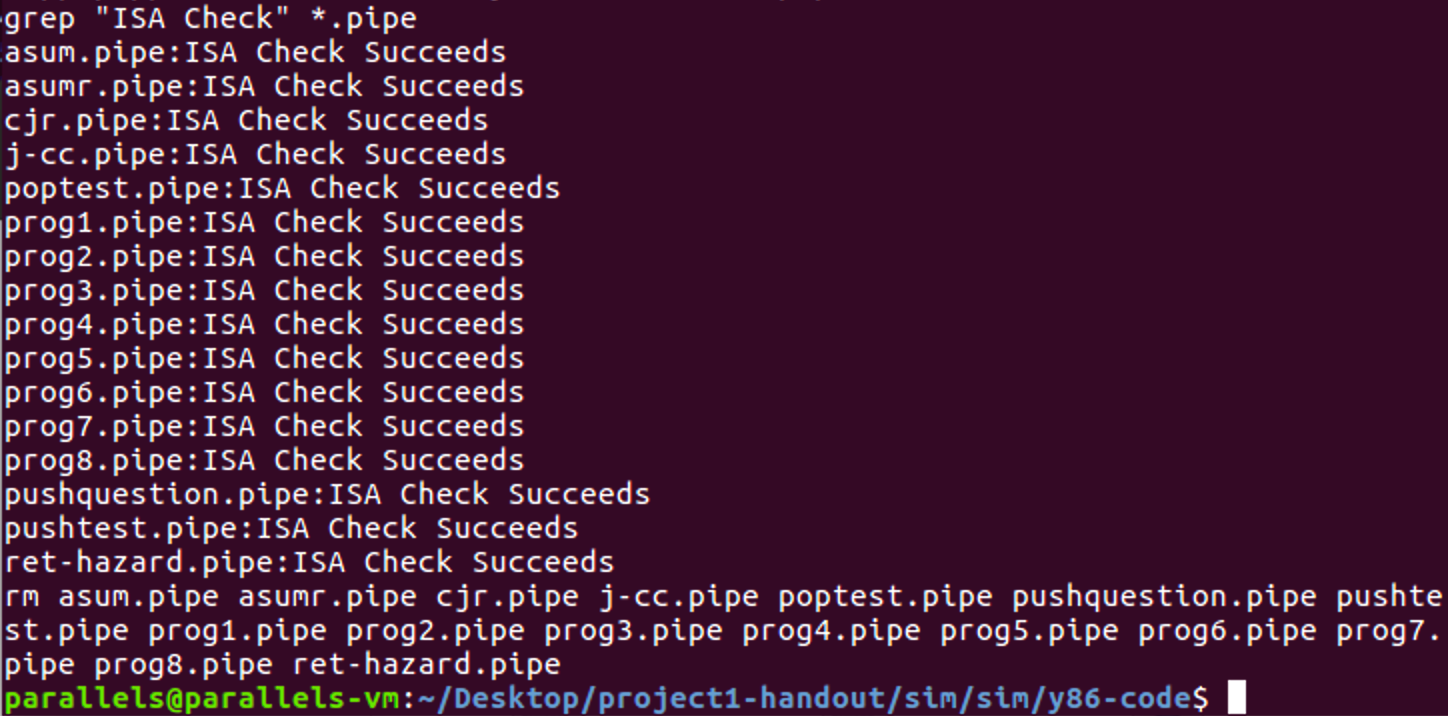
\includegraphics[width=1\textwidth]{benchmark_test.png}
		\caption{Testing pipeline simulator on the benchmark programs} \label{Fig-G11}
		\hspace{5mm}	
	\end{minipage}
\end{figure}
\begin{figure}[H]	
	\begin{minipage}[h]{\textwidth}	
		\centering
		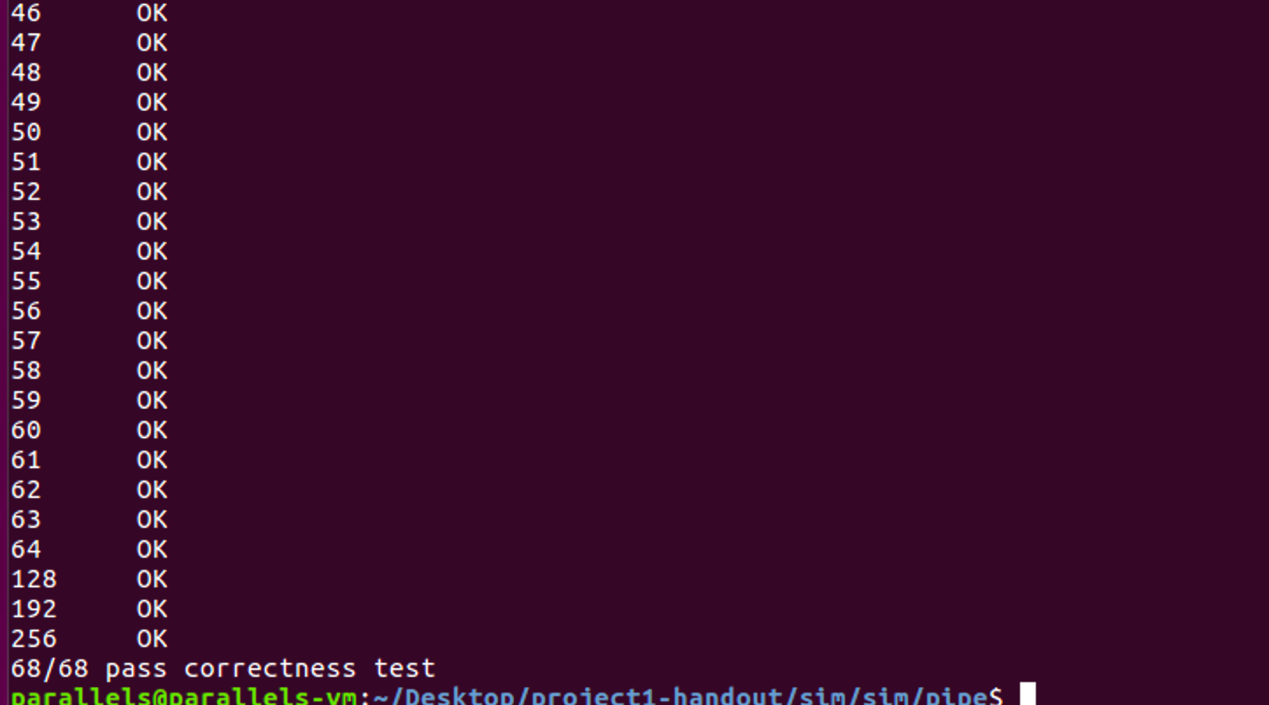
\includegraphics[width=1\textwidth]{range_block_pipeline.png}
		\caption{Testing code on a range of block lengths with the pipeline simulator} \label{Fig-G12}
		\hspace{5mm}
		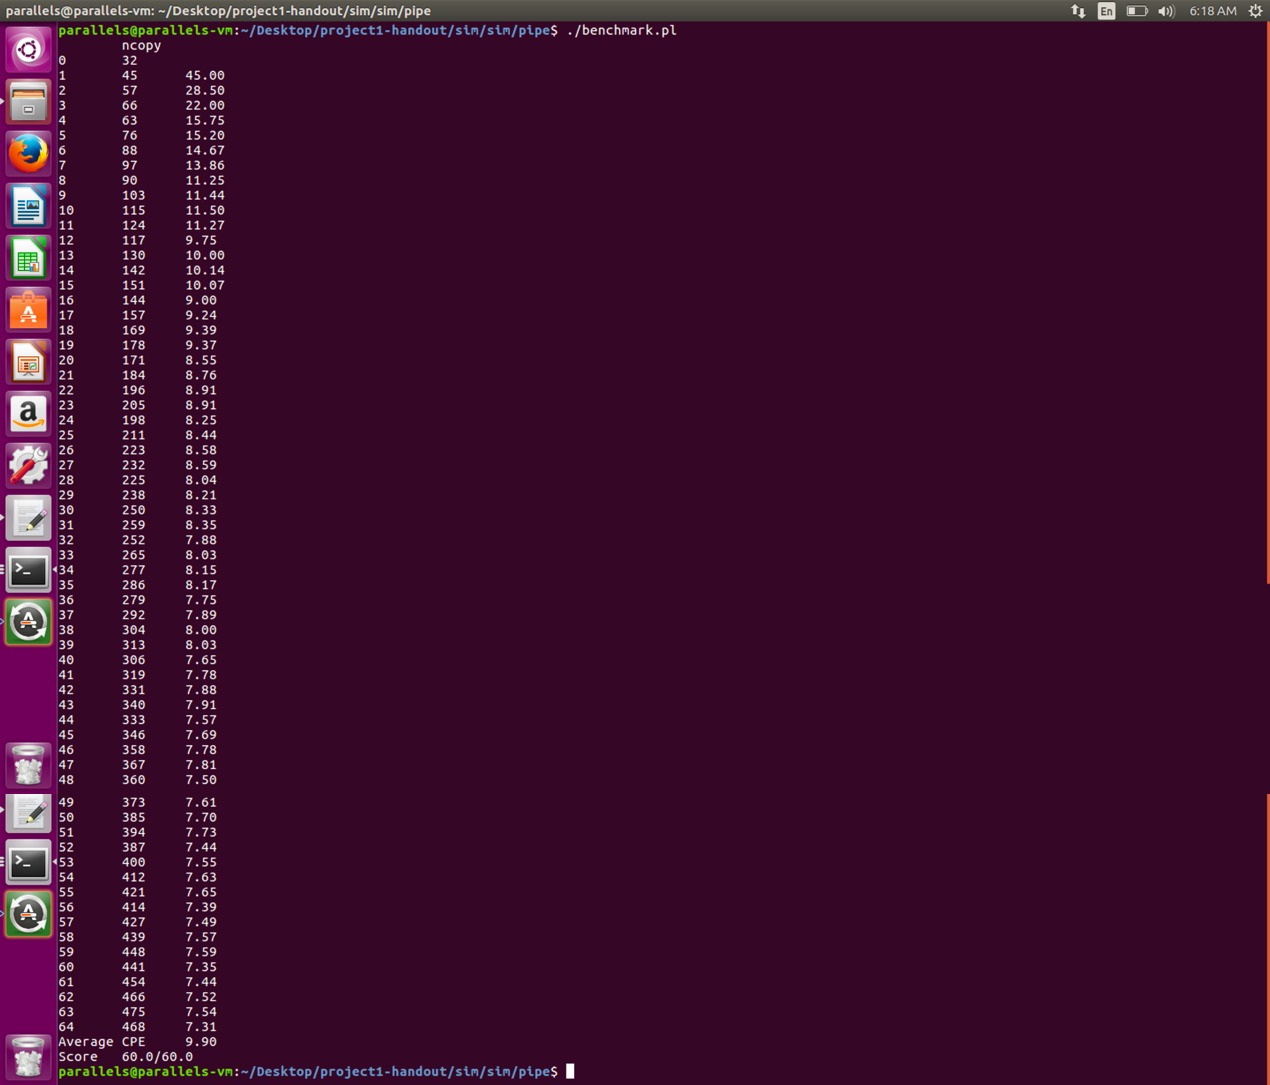
\includegraphics[width=1\textwidth]{performance_test.jpg}
		\caption{Performance test} \label{Fig-G13}
		\hspace{5mm}	
	\end{minipage}
\end{figure}

\section{Conclusion}

\subsection{Problems}

\textcircled{1}Installing issue\\
\begin{figure}[H]
	\begin{minipage}[h]{\textwidth}
		\centering
		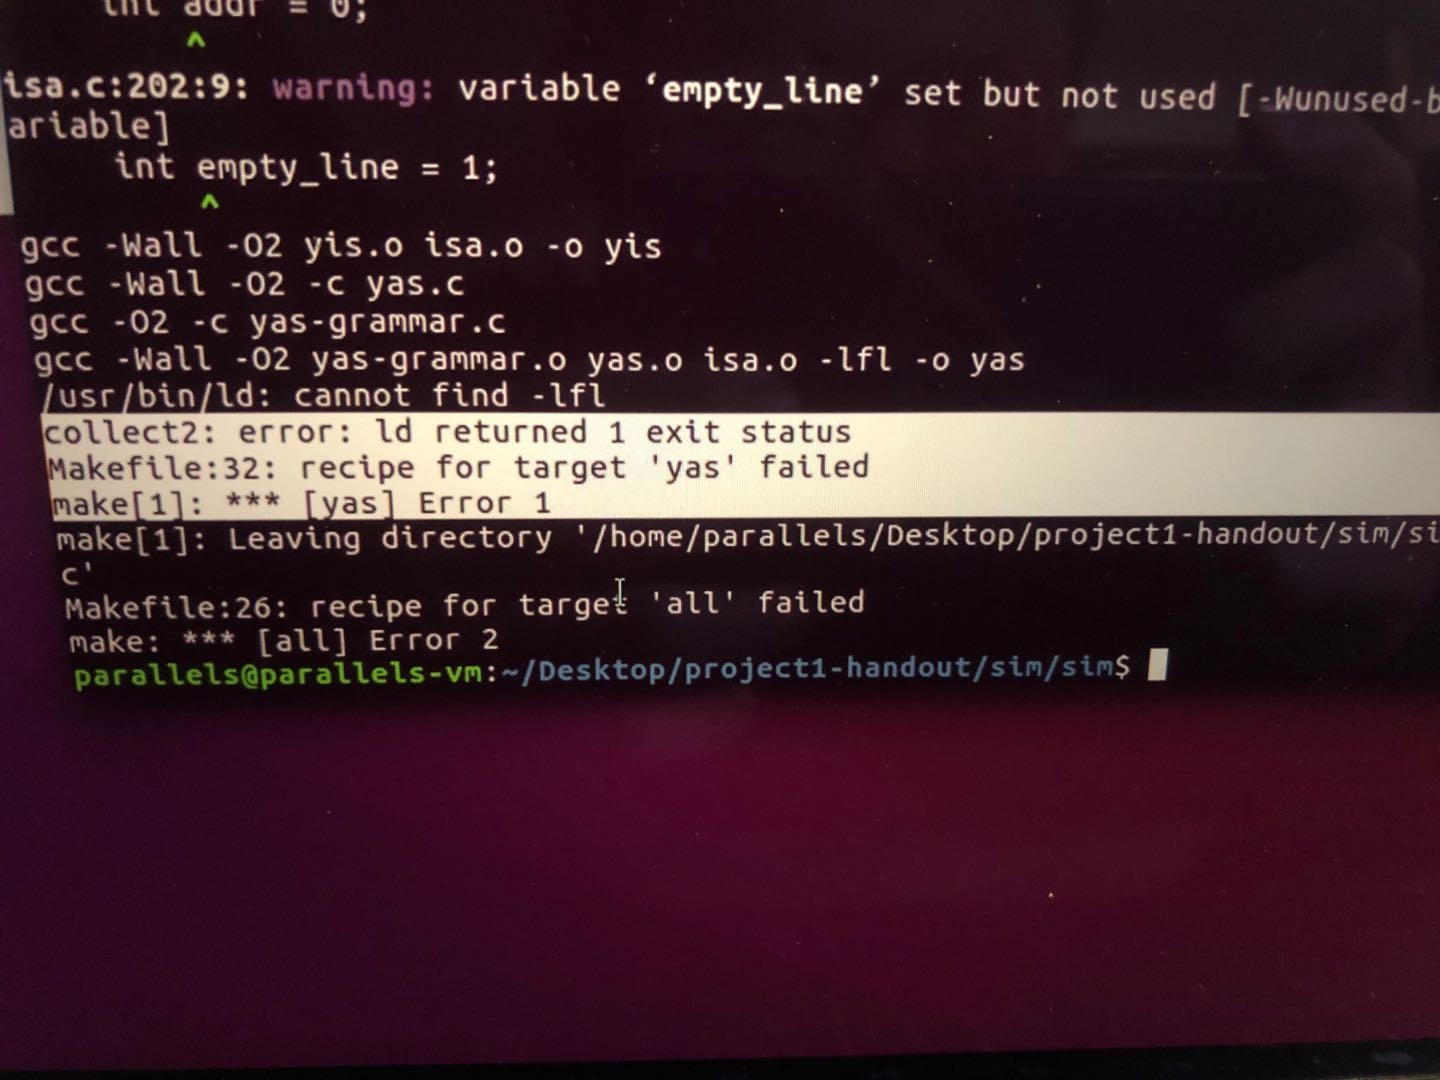
\includegraphics[width=0.6\textwidth]{problem1.jpg}
		\caption{Installing issue} \label{Fig-G14}
	\end{minipage}
\end{figure}
\textbf{Solution}: Using sudo apt-get install flex bison command to install flex and bison.\\
\textcircled{2}Modifying .hcl file\\
\begin{figure}[H]
	\begin{minipage}[h]{\textwidth}
		\centering
		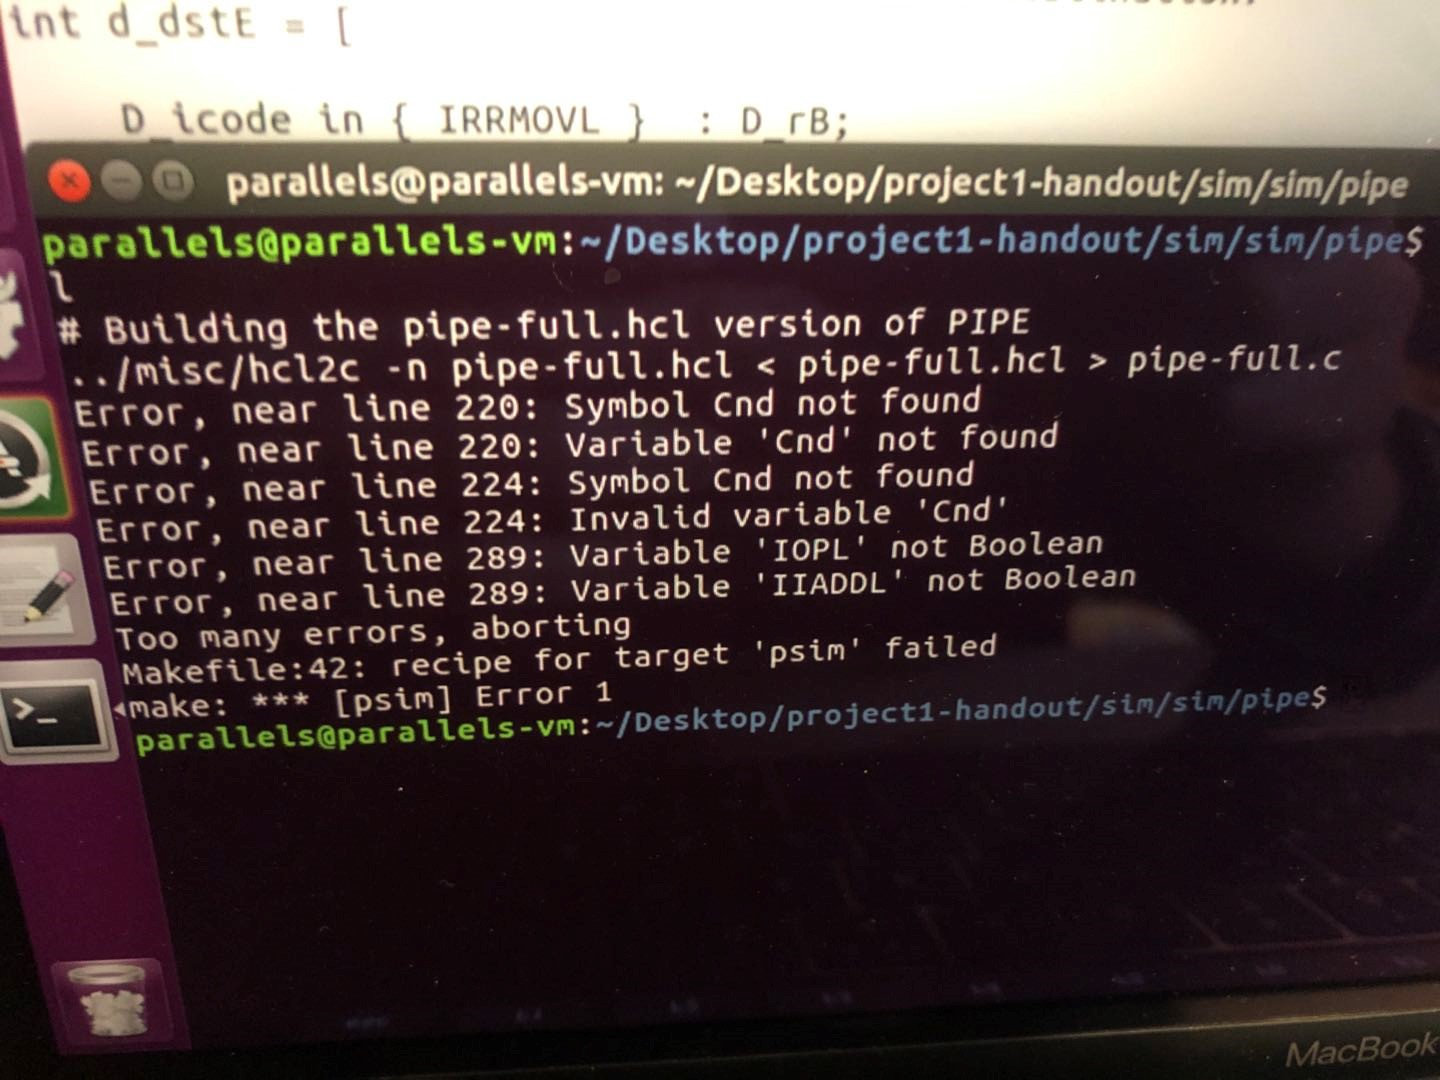
\includegraphics[width=0.6\textwidth]{problem2.jpg}
		\caption{Modifying issue} \label{Fig-G15}
	\end{minipage}
\end{figure}
\textbf{Solution}: The name of the variable is different. Cnd is changed to e\_Cnd. Set CC should be modified as\textbf{E\_icode in \{ IOPL, IIADDL \} \&\& !m\_stat in \{ SADR, SINS, SHLT \} \&\& !W\_stat in \{ SADR, SINS, SHLT \}}\\
\textcircled{3}matherr when make psim
\begin{figure}[H]
	\begin{minipage}[h]{\textwidth}
		\centering
		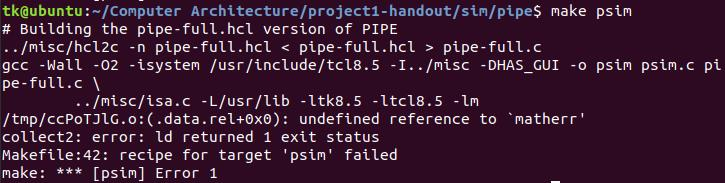
\includegraphics[width=0.6\textwidth]{problem3.jpg}
		\caption{matherr issue} \label{Fig-G16}
		\hspace{5mm}
		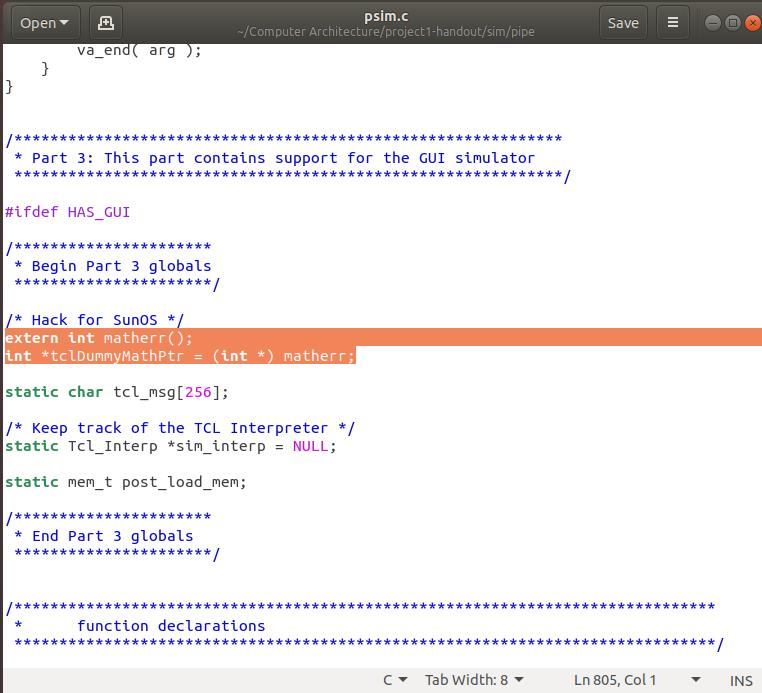
\includegraphics[width=0.6\textwidth]{solution3.jpg}
		\caption{matherr solution} \label{Fig-G13}
	\end{minipage}
\end{figure}
\textbf{Solution}: In \textbf{psim.c} remove 2 lines related to matherr.
\subsection{Achievements}

From this project, we mainly learn the following things:\\
\textcircled{1}Write and simulate the Y86 programs.\\
\textcircled{2}Modify .hcl file, have a shallow understanding of the HCL Description of Control for Single Cycle and Pipelined Y86 Processor.\\
\textcircled{3}Have a deeper understanding of loop unrolling and how the performance changes with different unrolling factors.

\section{Reference}
Computer Systems A Programmers Perspective 2e\quad-Bryant$\cdot$ O'Hallaron\\
https://blog.csdn.net/lishichengyan/article/details/79511161\\
https://blog.csdn.net/qq\_34262582/article/details/105465658\\
%----------------------------------------------------------------------------------------


\end{document}